OpenID standardin ensimmäisen version on kehittänyt toukokuussa 2005 Brad Fitzpatrick [TODO: lähde]. Tuoreimman 2.0 version kehitys aloitettiin 2007 ja sen kehitys on edelleen aktiivista. Se on SAMLia rajoitetumpi protokolla, jonka tavoite on käyttäjätunnuksen käytön mahdollistaminen eri web-palveluissa. Nykyään sen kehityksestä vastaa OpenID Foundation -säätiö, jonka jäsenenä on mm. Google ja Microsoft [TODO: lähde].

OpenID-palveluntarjoaja tarjoaa päätepisteen (endpoint), johon web-palvelut voivat tunnistautua. Tunnistautumiseen voidaan käyttää kahta erilaista virtausta (flow).  Suunnatussa identiteetin (directed identity) virtauksessa käyttäjä valitsee palveluntarjoajan, jonka kautta kirjautuminen suoritetaan [TODO: lähde]. Väitetyn identiteetin (claimed identity) virtauksessa web-palvelu hakee päätepisteen annetun OpenID-tunnisteen perusteella [TODO: lähde]. Virtaukset eroavat toisistaan vain vaiheessa, jossa etsitään päätepiste. Kuvassa \ref{openid_flow} on esitetty OpenID-kirjautumisen vaiheet.

\begin{figure}[ht]
\centering
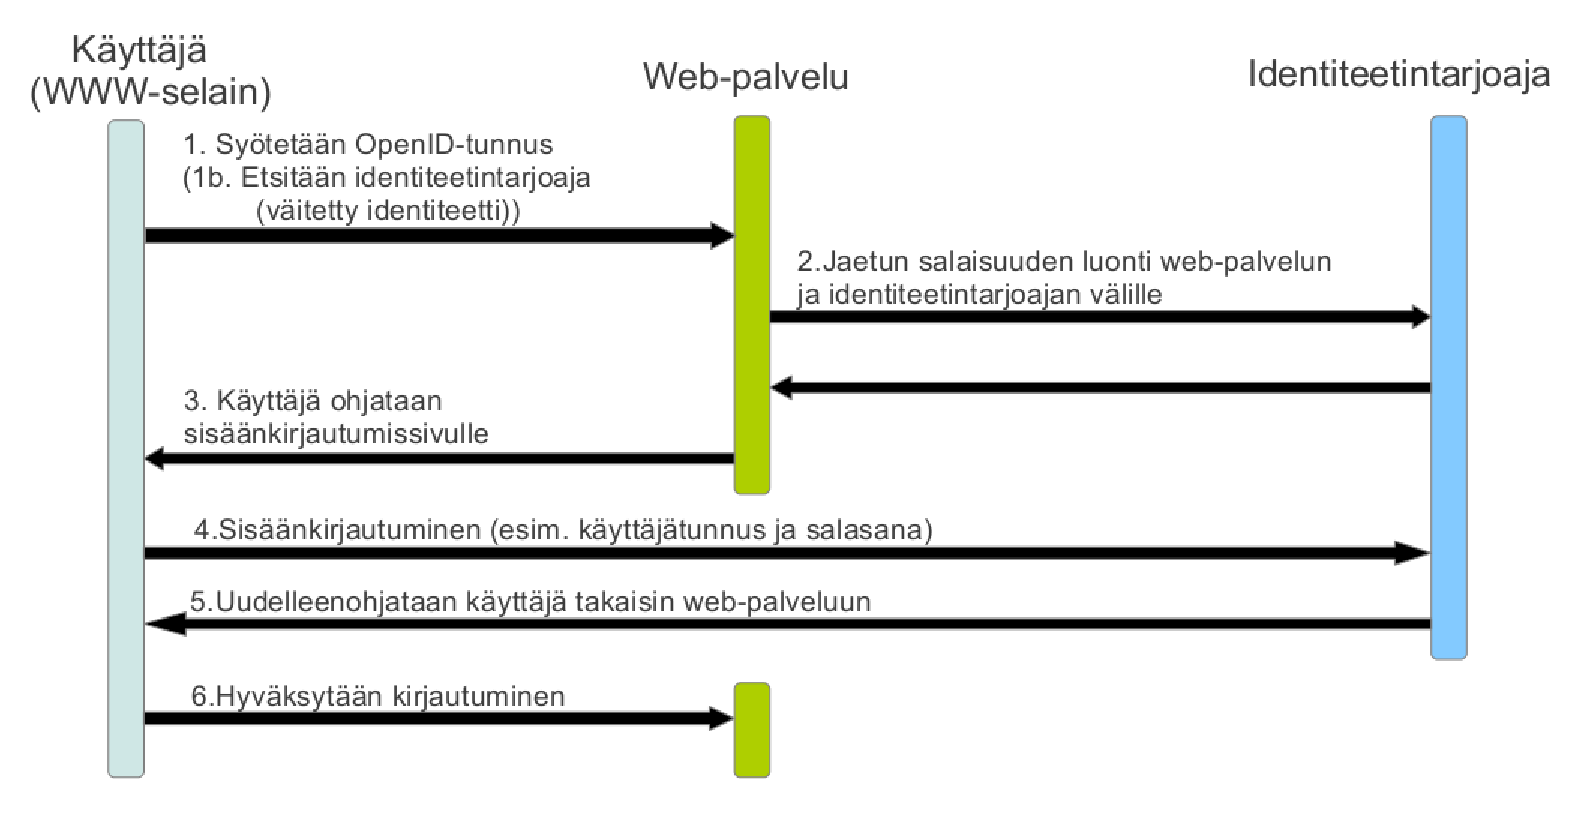
\includegraphics[width=\textwidth]{teknologiat/protokollat/openid.eps}
\caption{OpenID kirjautumisen vaiheet \cite{openid}.}%
\label{openid_flow}
\end{figure}

OpenID:n suhteen odotukset olivat alkujaan suuria, mutta myöhemmin into protokollan ympärillä on laantunut [TODO: lähde]. Esimerkiksi Microsoft vuonna 2008 aloittama OpenID-kokeilu on sittemmin lopetettu ja Microsoft on siirtynyt käyttämään omaa tunnistautumistoteutusta [TODO: lähde]. Yleiset OpenID-kirjautumissivut on korvattu eri palveluntarjoajien kirjautumissivuilla, koska käyttäjätutkimusten mukaan käyttäjät eivät tunne OpenID:tä, mutta tuntevat palveluntarjoajan kuten Googlen tai Yahoon [TODO: lähde]. Näin ollen käyttäjät eivät tiedä kirjautuvansa OpenID:llä palveluun, johon kirjaudutaan Googlen tunnuksilla. Myös alkuperäinen ajatus siitä, että kuka tahansa voi toimia identiteetintarjoajana, on osoittatunut toimimattomaksi, koska web-palveluiden ylläpitäjät haluavat luottaa päätepisteisiin, joiden kautta heidän palveluun voi kirjautua [TODO: lähde].

OpenID:tä lähellä on erillinen OAuth-protokolla, jonka toteutus aloitettiin, kun huomattiin ettei OpenID sovellu kaikkiin tapauksiin. OpenID:stä on kehittynyt myös OpenID Connect, joka paikkaa OpenID:n puutteita [TODO: lähde]. Sen kehitys on kuitenkin vielä niin varhaisessa määrittelyvaiheessa, että sen käyttö tämän tutkielman puitteissa ei ole mielekästä. Sen sijaan OAuth-protokolla on esitelty seuraavassa aliluvussa.